\chapter{Raccolta dati}

In questo capitolo approfondiamo le modalità di acquisizione definite per l'acquisizione dei dati, a partire dallo sviluppo di un interfaccia ad-hoc in Python per presentare i video previsti dal protocollo e somministrare tutti i questionari definiti, e la gestione della cattura e il salvataggio opportuno di tutti i dati e i segnali richiesti quali le espressioni facciali, la registrazione dello schermo, i dati di eye-tracking e i dati fisiologici.

\section{Sviluppo dell'interfaccia}

Per facilitare la fase di sperimentazione e raccolta dei dati è stato predisposto lo sviluppo di un'interfaccia, che guida il partecipante attraverso l'esperimento. L'interfaccia tiene traccia di tutte le acquisizioni effettuate, e in base al numero del partecipante, mostra i video previsti dal protocollo per tale partecipante, somministra i questionari definiti, e gestisce la cattura, il salvataggio e la sincronizzazione di tutti i segnali e i dati previsti, interfacciandosi con l'eye-tracker e il braccialetto Empatica\footnote{Insieme all'interfaccia è fornito uno script per il download automatico dei dati catturati dal braccialetto Empatica. Questo viene approfondito nel Paragrafo \ref{sec:download_empatica_data}}. L'interfaccia è stata sviluppata in Python, per mantenere il programma cross-platform, non essendo sicuri a monte del sistema operativo su cui si sarebbe fatto girare l'applicativo in fase di sperimentazione. L'interfaccia è stata sviluppata utilizzando la libreria di interfaccia grafica PyQt5. Il codice prodotto è reperibile al seguente link: \url{https://github.com/cosfederico/Interfaccia-Tesi/}.

\subsection{Design di sviluppo}

L'interfaccia è stata disegnata per essere controllata autonomamente dal partecipante. Una volta eseguita la calibrazione dell'eye-tracker (che deve essere svolta manualmente da un operatore), il partecipante è in grado di svolgere autonomamente l'esperimento, inserendo i propri dati e rispondendo alle domande proposte. Tutte le domande sono poste su una scala da 1 a 5, o in modalità a risposta multipla per le domande di comprensione, per cui il partecipante ha bisogno solo del mouse per interagire con l'interfaccia. È stato molto importante rendere l'interfaccia compatibile a un utilizzo a una sola mano, poiché su uno dei due polsi del partecipante (il polso della mano non dominante) è indossato il braccialetto Empatica per la misura del battito cardiaco e il livello di sudorazione. È caldamente consigliato da Empatica evitare di muovere tale polso per ottenere i risultati più accurati, per questo motivo è stata fatta tale scelta di design.

\subsection{Selezione dei video}

L'interfaccia gestisce autonomamente la selezione dei video da mostrare al partecipante corrente. Utilizzando lo storico delle acquisizioni eseguite sino a quel momento, l'interfaccia tiene conto del numero del partecipante attuale, e programmaticamente calcola i due video da somministrare a partire da tale numero, costruendo dinamicamente la matrice sperimentale presentata nella Sezione \ref{sec:variabili_indipendenti}, di cui è visibile un esempio in Tabella \ref{tab:matrice_sperimentale}.

Come già presentato in tale sezione, possiamo identificare univocamente un video tramite la valorizzazione di tra variabili binarie, quali $Contenuto$, $Tipo$ e $Genere$, le quali rappresentano rispettivamente:
\begin{itemize}
    \item $Contenuto$: il contenuto trattato, se A o B
    \item $Tipo$: il tipo di video, se Reale o Sintetico
    \item $Genere$: il genere del docente, se Maschile o Femminile
\end{itemize}

Andiamo a codificare le tre variabili indipendenti come variabili binarie con dominio $D_{Contenuto} = D_{Tipo} = D_{Genere} = \{0,1\}$, dove:

$$
Contenuto = 
     \begin{cases}
       0 &\quad\text{se il video contiene il Contenuto A} \\
       1 &\quad\text{se il video contiene il Contenuto B} \\
     \end{cases}
$$

$$
Tipo = 
     \begin{cases}
       0 &\quad\text{se il video è Reale} \\
       1 &\quad\text{se il video è Sintetico} \\
     \end{cases}
$$

$$
Genere = 
     \begin{cases}
       0 &\quad\text{se il genere del docente è Maschile} \\
       1 &\quad\text{se il genere del docente è Femminile} \\
     \end{cases}
$$

Una valorizzazione di queste tre variabili rappresenta un possibile video da somministrare al nostro partecipante. La matrice è costruita tale per cui il valore delle variabili associate al secondo video è calcolato mediante la negazione logica dei valori delle variabili associate al primo video, questo per garantire il controbilanciamento. Per questo motivo, il calcolo è eseguito per determinare il primo video da essere visionato. I risultati ottenuti per il primo video sono poi negati per ottenere le proprietà del secondo video da mostrare.

Il calcolo è basato su tre operazioni binarie. Trattando il numero del partecipante come un numero binario, sono estratti, in ordine, i tre bit meno significativi. Ad esempio, per un partecipante di numero 6, questo codificato in binario risulta:

\begin{align}
    \begin{split}
             &6_{10} = \underbrace{110} \\
         &\begin{array}{c}
            Contenuto = 0 \\
            Tipo = 1 \\
            Genere = 1
         \end{array}
    \end{split}
\end{align}

Nel caso del partecipante numero 14, sono ignorati i bit in eccesso:

\begin{align}
    \begin{split}
             14_{10}& = {1\underbrace{110}} \\ 
         &\begin{array}{c}
            Contenuto = 0 \\
            Tipo = 1 \\
            Genere = 1
         \end{array}
    \end{split}
\end{align}

Come si può evincere, in questo caso particolare i partecipanti 6 e 14 visioneranno gli stessi video, nello stesso ordine, rimarcando la natura periodica della matrice sperimentale.

Il calcolo esplicitato, per un generico partecipante di numero $ID_{partecipante}$, può essere scritto come:

\begin{align}
    \text{Contenuto} &= ID_{\text{partecipante}} \mod 2 \\
    ID_{\text{partecipante}} &\leftarrow \lfloor ID_{\text{partecipante}} / n \rfloor \\
    \text{Tipo} &= ID_{\text{partecipante}} \mod 2 \\
    ID_{\text{partecipante}} &\leftarrow \lfloor ID_{\text{partecipante}} / n \rfloor \\
    \text{Genere} &= ID_{\text{partecipante}} \mod 2
\end{align}

Si può osservare che non vi è in realtà alcun limite al numero di contenuti diversi che si potrebbero trattare, per cui la variabile contenuto non è limitata a essere binaria. In tal caso il calcolo per il contenuto da mostrare diventerebbe, più genericamente:

\begin{align}
    \begin{split}
        Contenuto &= ID_{partecipante} \mod k \\
        ID_{partecipante} &\leftarrow \lfloor ID_{partecipante} / k \rfloor \\
        &\dots
    \end{split}
\end{align}

dove $k$ è il numero di contenuti diversi trattati nello studio.

\subsection{Fase di preparazione}

L'interfaccia è stata arricchita di alcune funzionalità a supporto dello sperimentatore. Prima di cominciare con l'esperimento, viene aperta una finestra di preparazione, dove è possibile selezionare tra tutte le webcam attive sul sistema quale utilizzare per la registrazione del video, ed è presente un pulsante per effettuare una prova del sistema audio, per assicurarsi di avere selezionato l'uscita audio corretta (Figura \ref{fig:webcam_selection_screen}). A seguire, è visualizzata una finestra di anteprima della webcam selezionata. In sovra-impressione all'anteprima della webcam è posta una figura stilizzata per indicare il posizionamento ottimale della persona e del volto nell'inquadratura, per l'analisi ottimale delle espressioni facciali (Figura \ref{fig:webcam_preview_screen}). Terminata la fase di preparazione, viene lanciato il programma principale, dove il partecipante è accolto nella schermata di introduzione (Figura \ref{fig:welcome_screen_interfaccia}), dove è informato sui dettagli dell'esperimento, quali durata dei video e dell'esperimento, dati e segnali raccolti, e accorgimenti sull'utilizzo del mouse. Qui, il partecipante ha la possibilità di esprimere il suo consenso informato, tramite checkbox, e avviare l'esperimento, altrimenti uscire e abbandonare l'esperimento. L'avvio della registrazione di tutti i dati e segnali avviene solo una volta che il partecipante ha espresso il suo consenso e premuto il pulsante "Inizia". A partire da quel momento, l'esperimento è ufficialmente iniziato.

\begin{figure}[t]
    \centering
    \begin{subfigure}{0.49\textwidth}
        \centering
        \frame{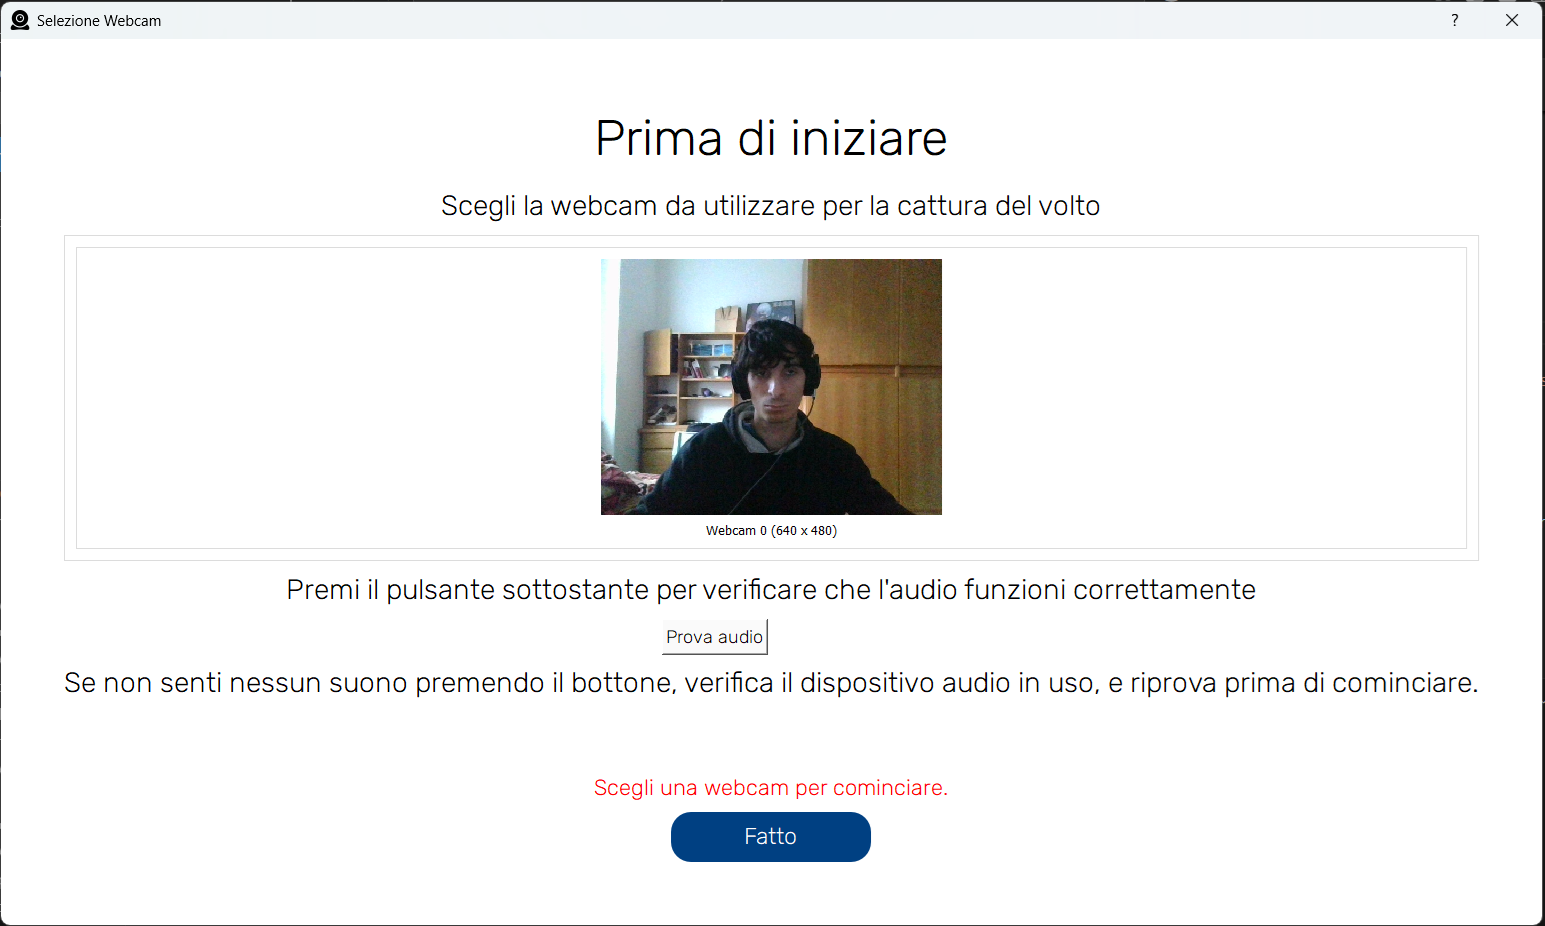
\includegraphics[width=\linewidth]{images/webcam_selection_screen}}
        \caption{}
        \label{fig:webcam_selection_screen}
    \end{subfigure}
    \hfill
    \begin{subfigure}{0.49\textwidth}
        \centering
        \frame{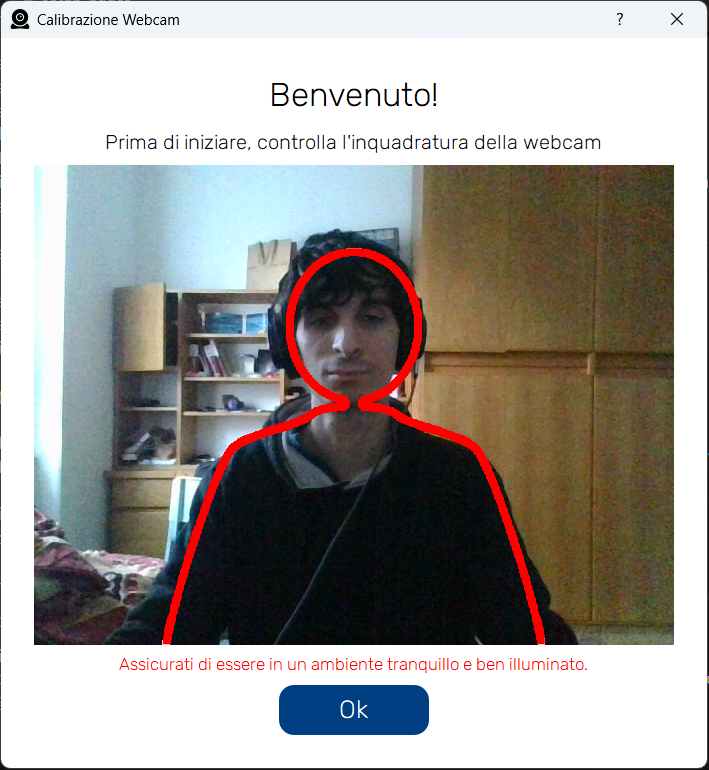
\includegraphics[width=0.55\linewidth]{images/webcam_preview_screen}}
        \caption{}
        \label{fig:webcam_preview_screen}
    \end{subfigure}
    \hfill
    \caption{Schermate di preparazione dell'interfaccia sviluppata: (a) Schermata di selezione della webcam. (b) Schermata di anteprima della webcam, con figura in sovra-impressione per il posizionamento ottimale del volto.}
    \label{fig:interfaccia_setup_windows}
\end{figure}

\begin{figure}[t]
    \centering
    \frame{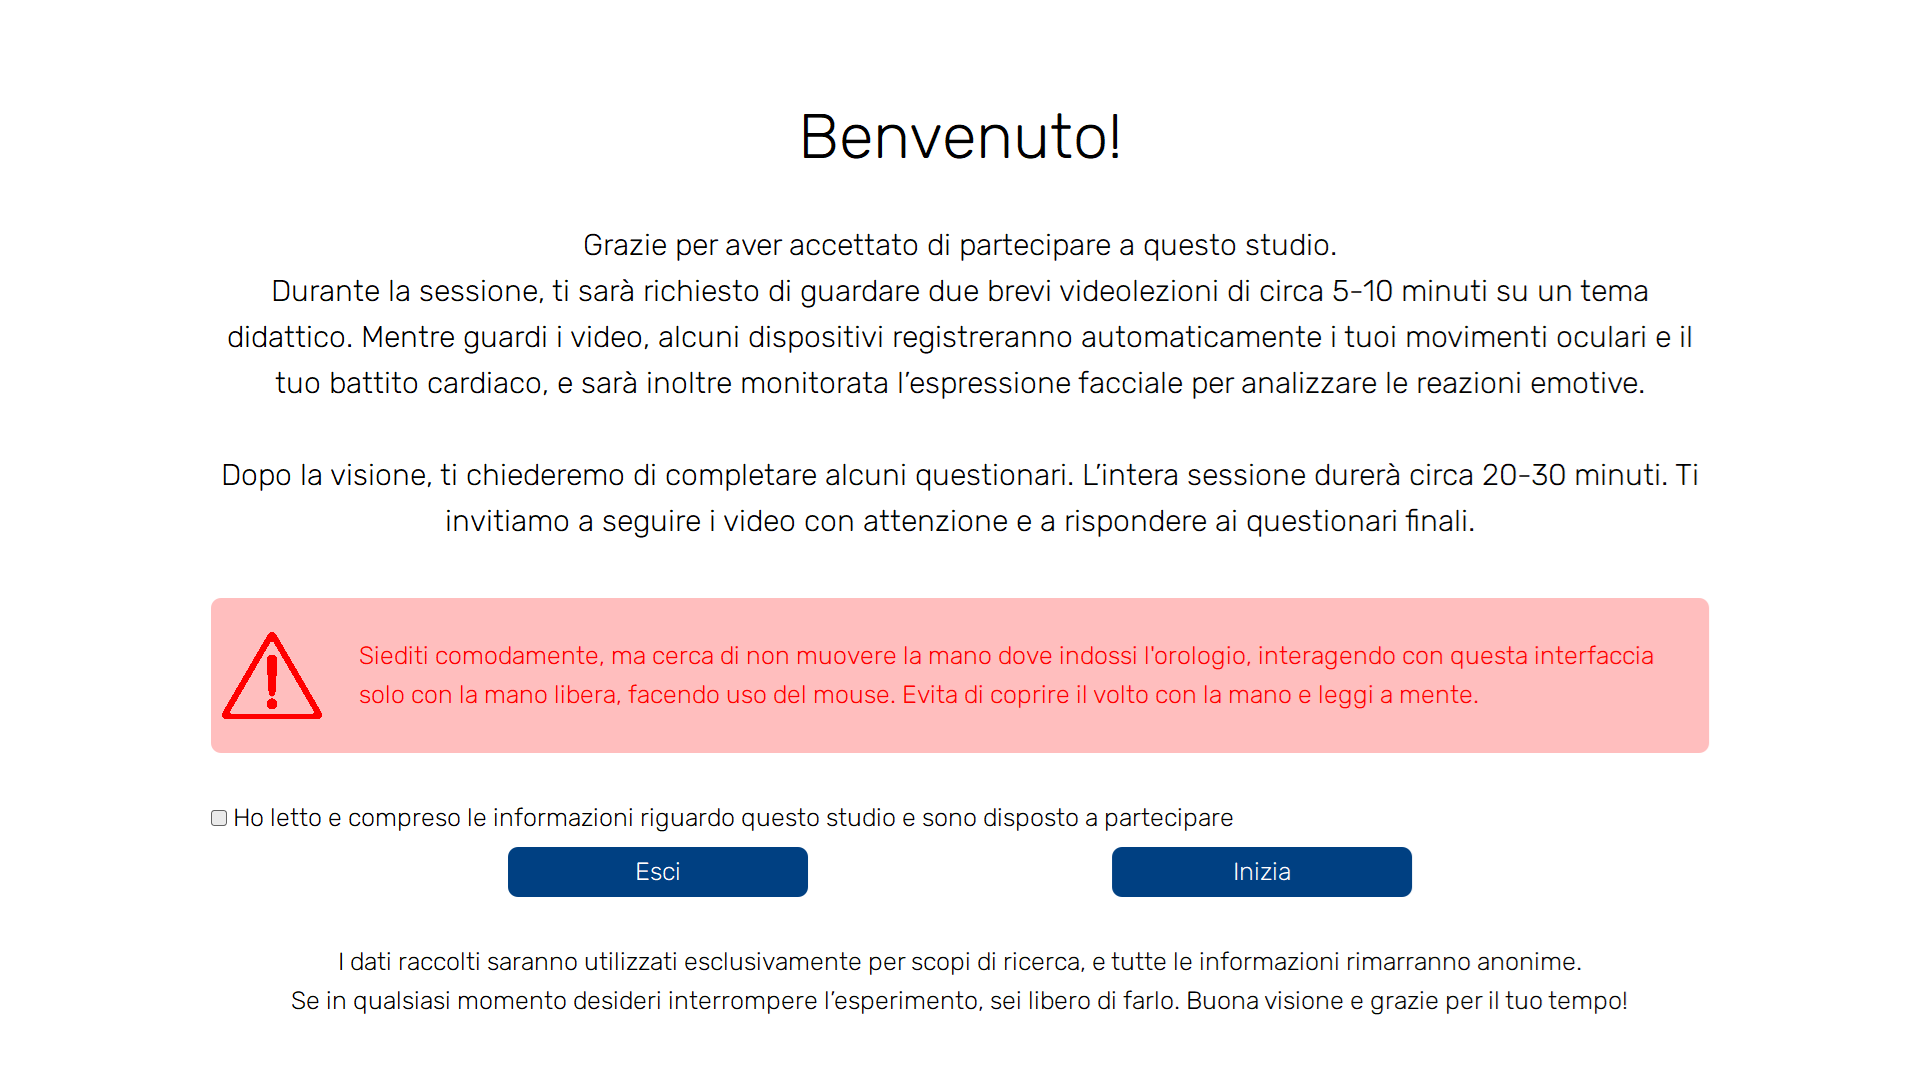
\includegraphics[width=\linewidth]{images/welcome_screen_interfaccia}}
    \caption{Schermata di benvenuto dell'interfaccia sviluppata.}
    \label{fig:welcome_screen_interfaccia}
\end{figure}

\subsection{Raccolta dei timestamp}

L'interfaccia tiene traccia di tutti i timestamp degli eventi principali, per permettere la sincronizzazione dei dati e dei segnali raccolti, e per poter associare i dati agli eventi di interazione del partecipante con l'interfaccia. L'interfaccia è stata disegnata a pagine: ogni volta che il partecipante passa alla pagina successiva viene salvato il timestamp di tale evento. In questo modo, sono salvati i timestamp di inizio sessione, fine sessione, inizio e fine di ogni video visualizzato, e i timestamp di risposta ad ogni domanda dei questionari presentati. I questionari sono stati disegnati in modo da presentare una domanda alla volta per pagina\footnote{Fatta eccezione per il questionario di autovalutazione dello stato emotivo (Positive and Negative Affect Schedule, PANAS), il quale è presentato in una pagina sola, e di questo è salvato solo il timestamp di inizio e fine di tutto il questionario.}: quando il partecipante passa alla domanda successiva, viene salvato il timestamp di tale evento. Questo ci permette non solo di sapere quando il partecipante è passato alla domanda successiva, ma anche quanto tempo  ha impiegato per rispondere alla domanda proposta, sottraendo il timestamp salvato con il precedente. Trattandosi di domande a risposta chiusa (da 1 a 5, o a risposta multipla) non ci si deve preoccupare del tempo di digitazione della risposta, in quanto per rispondere basta un click. I timestamp sono salvati in UNIX-time, rispetto al fuso orario UTC (Coordinated Universal Time).

\subsection{Registrazione della webcam/dello schermo}

Durante tutta la durata dell'esperimento, l'interfaccia si occupa della registrazione della webcam per l'estrazione delle espressioni facciali, e della registrazione dello schermo. 

\paragraph{Registrazione della webcam}
La registrazione del volto è effettuata tramite una webcam esterna, posta sotto al monitor sul quale sono presentati gli stimoli, e come già detto in fase di avvio l'interfaccia permette di selezionare quale webcam utilizzare per la registrazione del volto. Una volta selezionata, è mostrata allo sperimentatore una schermata con le istruzioni necessarie per il posizionamento ottimale della webcam (Fig. \ref{fig:webcam_preview_screen}).

\paragraph{Registrazione della webcam}
La registrazione dello schermo è necessaria per l'utilizzo dei dati di eye-tracking, in quanto rappresenta gli stimoli presentati. Combinando i dati di eye-tracking e la registrazione dello schermo è possibile analizzare il movimento dello sguardo e le fissazioni, associando ad ogni sguardo e fissazione lo stimolo sullo schermo che lo ha stimolato.

Le registrazioni sono eseguite su due processi paralleli al processo principale di generazione della GUI. Questo permette di non rallentare l'interfaccia grafica e permette una registrazione di entrambi i video più fluida, riducendo di molto il rischio di fotogrammi persi.

\subsection{Controllo dell'eye-tracker}

L'interfaccia si occupa anche del controllo dell'eye-tracker, e quindi dell'acquisizione e del salvataggio dei dati di eye-tracking. Questo è collegato al computer che esegue l'interfaccia tramite cavo Ethernet, ed è controllato utilizzando le librerie di API fornite dal produttore dell'eye-tracker.

A inizio esperimento, l'interfaccia effettua il collegamento con l'eye-tracker e avvia la procedura di calibrazione. La calibrazione è svolta manualmente dallo sperimentatore, il quale guida il partecipante attraverso il processo, e, dovesse essere necessario, riesegue la calibrazione fino ad ottenere dei risultati abbastanza buoni per una buon tracciamento dello sguardo. Quando la calibrazione è conclusa, il controllo torna all'interfaccia (Fig. \ref{fig:welcome_screen_interfaccia}), da dove il partecipante può far iniziare l'esperimento.

Quando il partecipante preme il pulsante per iniziare l'esperimento, l'interfaccia avvia la cattura dei dati di eye-tracking, gestendo il salvataggio del timestamp di inizio cattura, per permettere poi la sincronizzazione dei dati di eye-tracking con tutti gli altri dati.

\section{Salvataggio dei dati raccolti}

In questa sezione andiamo ad analizzare brevemente come tutti i dati raccolti dall'interfaccia vengono salvati, per essere poi pronti per la fase di analisi.

\subsection{Dati demografici e questionari}

I dati misti catturati dall'interfaccia, quali i dati demografici del partecipante (età, genere, nazionalità, livello di istruzione), le risposte ai questionari, e tutti i timestamp registrati, sono salvati in un formato \verb|.csv|. Il file \verb|.csv| presenta una sola riga, con campi:
\begin{itemize}
    \item ID del partecipante
    \item Dati demografici (età, genere, nazionalità, livello di istruzione)
    \item Timestamp di inizio, fine sessione
    \item Timestamp di inizio, fine video, natura e genere dei video mostrati
    \item Per ogni domanda la risposta selezionata e la domanda associata + timestamp
    \item Risposte ai questionari PANAS, con punteggio ottenuto + timestamp
    \item Risposte alle domande a risposta multipla, salvando la domanda chiesta, la risposta segnata, e se questa era corretta o meno + timestamp.
\end{itemize}

\subsection{Video}

Per l'estrazione delle espressioni facciali (registrazione della webcam) e l'analisi degli stimoli visivi (registrazione dello schermo) non è necessario l'utilizzo del segnale RAW della webcam, per cui le registrazioni sono salvate in formato \verb|.mp4| compresso, per ridurre lo spazio richiesto per memorizzare i dati salvati.

\subsection{Eye-tracking}

Come già detto, il sistema di eye-tracking è controllato internamente dall'interfaccia, utilizzando le API fornite da SR Research. A fine esperimento, l'interfaccia si occupa di interrompere l'acquisizione dei dati di eye-tracking e scaricare i dati registrati. I dati sono trasferiti via Ethernet, e sono scaricati in un formato proprietario (\verb|.edf|, Eyelink Data Format), ma Research SR fornisce un programma da linea di comando per convertire tale formato in formato di testo (\verb|.txt|). L'interfaccia si occupa quindi di scaricare i dati e convertirli in formato \verb|.txt|. Il file \verb|.txt| prodotto presenta una riga per campione, con posizione $x,y$ dello sguardo sullo schermo, e diametro della pupilla, in numero di pixel. Per l'analisi dei dati è stato sviluppato uno script per la conversione dei dati dal formato \verb|.txt| al formato \verb|.csv|. Nel Capitolo \ref{cap:data_analysis} verrà approfondito come questi dati sono utilizzati e come il diametro della pupilla è convertito da numero di pixel in $cm$.

\section{Dati fisiologici}
\label{sec:empatica}

Dedichiamo una breve sezione a parte per i dati fisiologici, i quali non sono controllati dall'interfaccia direttamente, bensì tramite applicazione via smartphone. 

\subsection{Setup}

Per l'acquisizione dei segnali fisiologici è stato scelto l'utilizzo di un braccialetto Empatica EmbracePlus. Il braccialetto, indossabile al polso come un normale orologio, permette l'acquisizione non invasiva dei segnali che ci interessano, quali il battito cardiaco e il livello di sudorazione della pelle, così come anche molto altri segnali. Il braccialetto non presenta delle API per il controllo diretto, ma è pilotato via un applicazione via smartphone. L'applicazione in questione è CareLab, prodotta da Empatica, e disponibile sia per iOS che per Android. Per potersi collegare all'orologio è necessario scaricare l'applicazione, effettuare il login, e solo allora il telefono è in grado di collegarsi al braccialetto tramite Bluetooth.

La generazione delle credenziali per accedere all'app è eseguita tramite un portale dedicato, fornito da Empatica a tutti i suoi clienti (\url{https://auth.carelab.empatica.com/}). Da questo portale, lo sperimentatore crea un "Partecipante": un partecipante non è altro che una coppia di credenziali (username e password), utilizzabili per effettuare l'accesso sull'app. Effettuato l'accesso sull'app, lo smartphone si collega all'orologio, mostrando le istruzioni per indossarlo correttamente, e avvia immediatamente l'acquisizione dei dati. Per la gestione dei dati acquisiti, è stato scelto di utilizzare un solo partecipante per raccogliere i dati associati alla sperimentazione. Il portale è condiviso tra tutti i dispositivi di un associazione, ed essendo il braccialetto utilizzato di proprietà dell'Università, è bene concentrare tutti i dati in un posto solo. Per la distinzione delle catture è stato utilizzato il tempo di inizio dell'esperimento, univoco per ogni acquisizione.

\subsection{Calibrazione}

\sloppy
Il braccialetto non prevede una particolare fase di calibrazione. Una volta collegato via app, è richiesto massimo un minuto di configurazione eseguita automaticamente. Detto questo, come consigliato dalle guide di Empatica (\url{https://support.empatica.com/hc/en-us/articles/203621955-What-should-I-know-to-use-EDA-data-in-my-experiment}), per la cattura e l'utilizzo del livello di sudorazione della pelle (o Electrodermal Activity, EDA), è consigliato indossare l'orologio in condizioni di riposo per circa 10-15 minuti prima dell'inizio dell'esperimento, per permettere alla pelle del partecipante di adattarsi al contatto con il sensore, e permettere l'acquisizione di un buon segnale di sudorazione.

\subsection{Acquisizione dei segnali}
\fussy

Dopo la fase di calibrazione, il braccialetto inizia subito a catturare dati. L'acquisizione è quindi automatica e asincrona. I dati vengono trasferiti continuamente sul telefono e sincronizzati periodicamente su un server Amazon AWS. Per questo motivo, è importante che la cattura dei dati fisiologici sia avviata e terminata rispettivamente prima e dopo che l'esperimento sia iniziato e finito, così da permettere di sincronizzare i segnali fisiologici con i dati raccolti dell'interfaccia.

\subsection{Salvataggio dei dati}

Una volta terminato l'esperimento, è presente sull'app un pulsante per interrompere l'acquisizione, il quale arresta l'acquisizione dei dati, trasferisce i dati non ancora sincronizzati, li carica sul cloud online e spegne l'orologio. A seguito di questa operazione, i dati sono al sicuro sul cloud, e sono scaricabili in qualsiasi momento, accedendo al cloud tramite le credenziali AWS, fornite da Empatica sul portale indicato. Questa soluzione è stata valutata come molto utile, in quanto, posto che l’orologio sia stato configurato correttamente, il salvataggio dei dati è automatico, non dovendosene preoccupare durante la sperimentazione.

\subsection{Download dei dati}
\label{sec:download_empatica_data}

Per il download dei dati dal cloud è stato sviluppato uno script in Python, che utilizzando l'ID del partecipante, l'ora dell'acquisizione e i dati di login al server AWS, scarica automaticamente i dati associati alla acquisizione e li sincronizza con la cattura, ritagliando i dati che ci servono. Questa operazione verrà approfondita nel Capitolo \ref{cap:data_analysis} sull'elaborazione dei segnali. Lo script si occupa anche di selezionare i segnali che si vogliono scaricare. Il braccialetto Empatica in realtà è in grado di catturare un gran numero di segnali, e in condizioni normali li cattura tutti. Questi segnali sono:
\begin{itemize}
    \item Accelerometro ($x,y,z$)
    \item Giroscopio ($x,y,z$)
    \item Temperatura della pelle (°C)
    \item \textbf{ElectroDermal Activity} ($\mu S$)
    \item Passi
    \item \textbf{Blood Volume Pulse (BVP)} ($nW$)
    \item \textbf{Systolic Peaks}
\end{itemize}
Tra questi sono indicati in grassetto i dati che vengono scaricati, quali: i dati di picchi sistolici (systolic peaks), per il battito cardiaco, il livello di sudorazione della pelle (ElectroDermal Activity, o EDA), e anche il segnale di BVP (volume di pressione nel sangue), il quale è sempre associato al battito cardiaco, e potrebbe tornare utile in fase di analisi. In verità, il braccialetto produce anche una serie di segnali aggregati, ovvero segnali più complessi come il battito cardiaco o il ritmo respiratorio, ma questi segnali sono aggregati per minuto, ovvero vi è un campione ogni minuto. Questo rende l'utilizzo di questi dati aggregati non applicabile per la nostra ricerca, la quale richiede una precisione più fine\footnote{Volendo analizzare il comportamento di questi segnali durante la visione di video, dalla durata media di 6-7 minuti, un dato aggregato per minuto ci è molto poco utile, il quale presenterebbe nel caso migliore 7 campioni per video, i quali tornano utili a molto poco}. I segnali indicati sono i cosidetti segnali RAW. Nel Capitolo \ref{cap:data_analysis} verrà approfondita l'analisi di questi segnali, e come questi segnali vengono utilizzati, ad esempio come il segnale di picchi sistolici viene utilizzato per ricostruire il segnale di battito cardiaco in forma non aggregata.

\clearpage